\documentclass[oneside,11pt]{article}
\usepackage[algo,french,url,dot]{my_package}

\title{\emph{myproof}\\projet de compilation}

\begin{document}

\maketitle

\begin{figure}[here]
  \centering
  \begin{dot2tex}[neato]
    digraph G
    {
      node [fixedsize=true, width=0.4, style="fill=green!20"];
      "myproof" -> {"gcc plugin" "profiler" "report"};
      "gcc plugin" -> {"init" "passes" "pragmas" "summary" "error" "end" "measure" "params"};
      "myproof" [style="fill=orange!80"];
      "gcc plugin" [style="fill=orange!40"];
    }
  \end{dot2tex}
  \caption{Hierarchy of main features}
  \label{fig:hierarchy}
\end{figure}

      % "passes" -> {"function pass" "basicblock pass" "loop pass" "bb pass" "variable pass" "instrumente pass"};
      % "pragmas" -> {"instrumente pragma"};
      % "summary" -> {"all data structures std output" "static instrumentation output"};
      % "error" -> {"checks existing instrumented function"};
      % "end" -> {"remove all data structures"};

      % "profiler" -> "python script";

\newpage

\tableofcontents

\newpage

\section{Introduction}

\emph{myproof} est un logiciel de profiling, à la manière de \emph{gprof}\footnote{GNU gprof: \url{http://www.cs.utah.edu/dept/old/texinfo/as/gprof_toc.html}}, regroupant toutes les étapes nécessaire à l'instrumentation et à la mesure d'une application cible. Il se différencie, tout de même, de ce dernier en apportant une interface modulable. En effet, il devient possible avec \emph{myproof} d'integrer aisément, par exemple, sa propre ``pass''\footnote{une pass gcc} ou encore un nouveau ``pragma''\footnote{\#pragma directive}. Pour cela, \emph{myproof} fournit des structures de données complètes comme ``les fonctions'', ``les blocs de base'', ``les boucles'' mais aussi ``les chemins'' entre blocs de base.

\subsection{Hierarchie des fonctionnalités principales}

Nous présentons, en figure \ref{fig:hierarchy}, les fonctionnalités principales de notre logiciel de profiling. En partant de la racine du projet, nous avons 3 sous-noeuds qui sont respectivement ``gcc plugin'', ``profiler'' et ``report''. ``gcc plugin'' est le repertoire contenant le plugin. Il permet de charger à chaud les fonctionnalités de ``myproof'' durant la phase de compilation de gcc. ``profiler'' contient l'outil de profiling. ``report'' est le repertoire contenant ce jolie rapport. Nous verrons plus en détail, par la suite, les fonctionnalités de ``gcc plugin''.

\begin{figure}[here]
  \centering
  \begin{dot2tex}[neato]
    digraph G
    {
      node [fixedsize=true, width=0.4, style="fill=green!20"];
      "myproof" -> {"gcc plugin" "profiler" "report"};
      "gcc plugin" -> {"init" "passes" "pragmas" "summary" "error" "end" "measure"};
      "myproof" [style="fill=orange!80"];
      "gcc plugin" [style="fill=orange!40"];
    }
  \end{dot2tex}
  \caption{Hierarchy of main features}
  \label{fig:hierarchy}
\end{figure}

      % "passes" -> {"function pass" "basicblock pass" "loop pass" "bb pass" "variable pass" "instrumente pass"};
      % "pragmas" -> {"instrumente pragma"};
      % "summary" -> {"all data structures std output" "static instrumentation output"};
      % "error" -> {"checks existing instrumented function"};
      % "end" -> {"remove all data structures"};

      % "profiler" -> "python script";


% \begin{figure}[here]
%   \centering
% \begin{dot2tex}[dot,tikz,codeonly,styleonly,options=-s -tmath]
%   digraph G {
%     d2tdocpreamble = "\usetikzlibrary{automata}";
%     d2tfigpreamble = "\tikzstyle{every state}= \
%     [draw=blue!50,very thick,fill=blue!20]";
%     node [style="state"];
%     edge [lblstyle="auto",topath="bend left"];
%     A [style="state, initial"];
%     A -> B [label=2];
%     A -> D [label=7];
%     B -> A [label=1];
%     B -> B [label=3,topath="loop above"];
%     B -> C [label=4];
%     C -> F [label=5];
%     F -> B [label=8];
%     F -> D [label=7];
%     D -> E [label=2];
%     E -> A [label="1,6"];
%     F [style="state,accepting"];
%   }
% \end{dot2tex}
%   \caption{Test a dot}
%   \label{fig:test2}
% \end{figure}

\subsection{CMake}

Il est important de noter que compte tenu des nombreuses parties que regroupe ce projet, il nous a semblé plus approrié d'utiliser CMake. Plus exactement il nous permet de lier toutes les parties de notre projet et crée des liens de dépendances entre elles toute en s'abstrayant des contraires de portabilité liées aux divergences des OS\footnote{Systèmes d'exploitation}.

\subsection{Le plugin GCC}

Pour ce qui concerne les différentes phases d'instrumentation, nous avons choisi de développer un plugin, ce qui permet d'enrichir les fonctionnalités de GCC sans pour autant avoir à le recompiler.

\begin{center}
  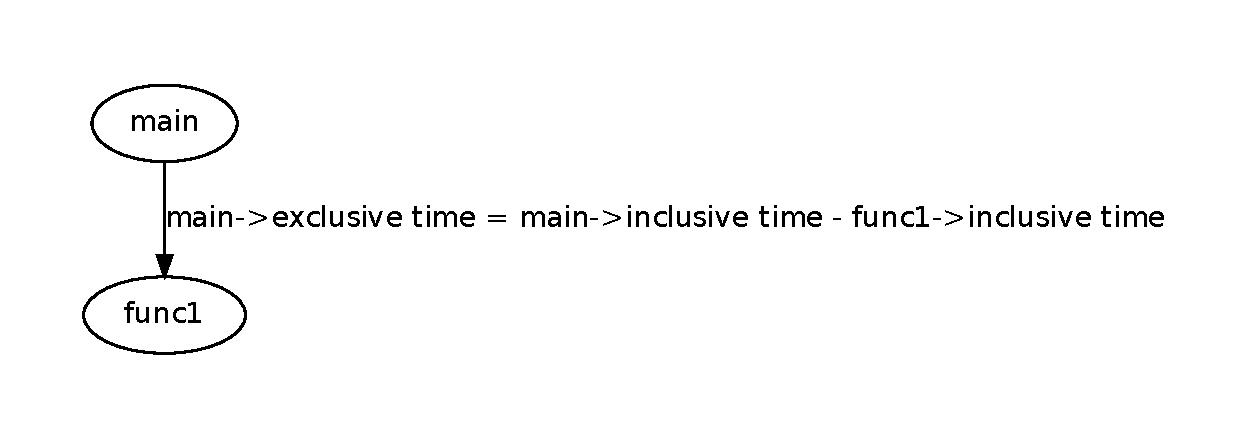
\includegraphics[scale=0.50]{images/tree2.pdf}
  \captionof{figure}{test2}
\end{center}

\begin{center}
  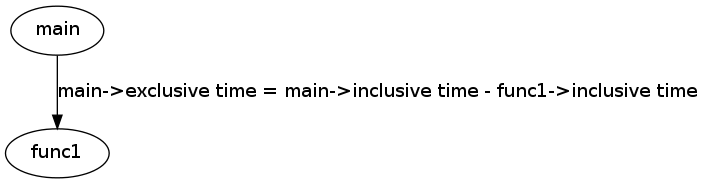
\includegraphics[scale=0.50]{images/tree.png}
  \captionof{figure}{test}
\end{center}


\newpage

\section{Instrumentation statique}

\subsection{La problématique}

La problématique de cette partie était de dresser un profil statique du code considéré, c'est-à-dire obtenir une trace des accès mémoire à la compilation. Un exemple est illustré en figure \ref{fig:static_result}.

\begin{figure}[here]
  \centering
\begin{verbatim}
 fonction toto
 3 load
 2 * N load
 1 * N store
 2 load
 3 * M load
 3 * M store
\end{verbatim}
  \caption{Résultat obtenu par l'instrumentation statique}
  \label{fig:static_result}
\end{figure}

\subsection{Accès mémoire}

Ces accès mémoire se traduisent par les instructions load et store exécutées. Nous considérons qu'une instruction load est détectée lorsque le contenu d'un tableau est affectée à une variable, un store lorsqu'un tableau récupère la valeur d'une variable.\\

\subsection{Blocs de base et boucles}

L'idée était donc de parcourir les blocs de base composant chaque fonction du code. La principale difficulté de cette phase de profiling consistait à détecter les éventuelles boucles présentes au sein d'une fonction, puis traiter les blocs de base, en évitant les redondances.

\subsection{Parsing des boucles et blocs de base}

Cette opération a été effectuée en deux passes: le parsing des boucles \verb#pass_loop#, puis celui des blocs de base courants \verb#pass_bb#.\\

Dans les 2 passes, l'instrumentation se déroule de la façon suivante:\\

\begin{itemize}

\item La fonction principale de la passe parcourt tous les blocs de base à l'aide de la macro \verb#FOR_EACH_BB#. Puis, elle utilise un itérateur pour analyser les ``statements'', c'est-à-dire les lignes du bloc de base courant. Ceci est fait grâce à la fonction \verb#read_stmt()#.\\

\item La fonction \verb#read_stmt()# qui est appelée permet de savoir si le statement correspond à un appel de fonction, un retour, une condition, ou plus simplement une affectation\footnote{voir ``GIMPLE\_ASSIGN'' dans gimple}. C'est ce dernier cas qui nous intéresse.\\

\item Ensuite, nous avons besoin de savoir de quel côté de l'égalité nous sommes. La fonction \verb#read_stmt()# nous donne également la position de l'opérande (à droite ou à gauche de l'égalité). La fonction \verb#read_operand()#, quant à elle, détermine le type rencontré, en l'occurence, celui qui nous intéresse\footnote{voir ``INDIRECT\_REF'' dans gimple}. Un exemple de code est fournit en figure \ref{fig:count_example}.\\

\item Lorsque ce cas est rencontré, on incrémente le compteur de loads si l'opérande est à droite de l'égalité, et le compteur de stores si l'opérande se trouve à gauche.\\

\end{itemize}

\begin{figure}[here]
  \centering
\begin{verbatim}
case INDIRECT_REF:
  /* pointer & dereferencing */
  if ( store == true ) { basicblock->nstore++; }
  else { basicblock->nload++; }
  break;
\end{verbatim}
  \caption{Exemple de code d'incrementation des compteurs de load et store}
  \label{fig:count_example}
\end{figure}

\subsection{La passe des boucles}

La première passe \verb#pass_loop# détecte les éventuelles boucles présentes dans la fonction instrumentée, en la parcourant. Elle stocke dans une structure les blocs de base contenus dans lesdites boucles.\\

La détection des boucles est possible grâce au code présenté en figure \ref{fig:pass_loop}, au sein de la fonction \verb#pass_loop()#.\\

\begin{figure}[here]
  \centering
\begin{verbatim}
if ( cfun->x_current_loops != NULL )
{
    read_loop( cfun->x_current_loops->tree_root, function );
}
\end{verbatim}
  \caption{Appel de la fonction read\_loop}
  \label{fig:pass_loop}
\end{figure}

La fonction \verb#read_loop()# permet de connaître les bornes des boucles rencontrées dans la fonction, et ainsi de multiplier le nombre des opérations éventuelles load et store par le nombre d'itérations de la boucle. Les blocs de base contenant ces boucles sont écartées du traitement classique des blocs, afin d'éviter des redondances.

\subsection{La passe des blocs de base}

La seconde passe \verb#passe_bb#, quant à elle, reparcourt les blocs de base de la fonction, et vérifie pour chaque bloc considéré s'il a déjà été traité dans la passe précédente. Dans ce cas, elle passe au bloc de base suivant. Dans le cas contraire, elle analyse chaque statement du bloc.

\subsection{Localisation des passes}

Au niveau de l'enregistrement de la passe \verb#pass_loop#, nous avons changé le paramètre ``mudflap2'' dédié au parcours GIMPLE, par ``parloops''.

\subsection{Paramètres d'optimisation}

Enfin, pour prendre en compte les boucles du code à compiler, les options d'optimisation ``-O1'' ou ``-O2'' de gcc doivent être utilisées.

\subsection{Graphe CFG}

Nous vous présentions précédement les blocs de base ainsi que les ``chemins'' entre blocs de base que ``myproof'' reconnait.\\

Il nous est donc possible de générer des graphes CFG\footnote{Grammaire non contextuelle}.\\

Nous vous présentons en figure \ref{fig:cfg} un exemple de graphe d'une fonction.

\begin{figure}[here]
  \centering
  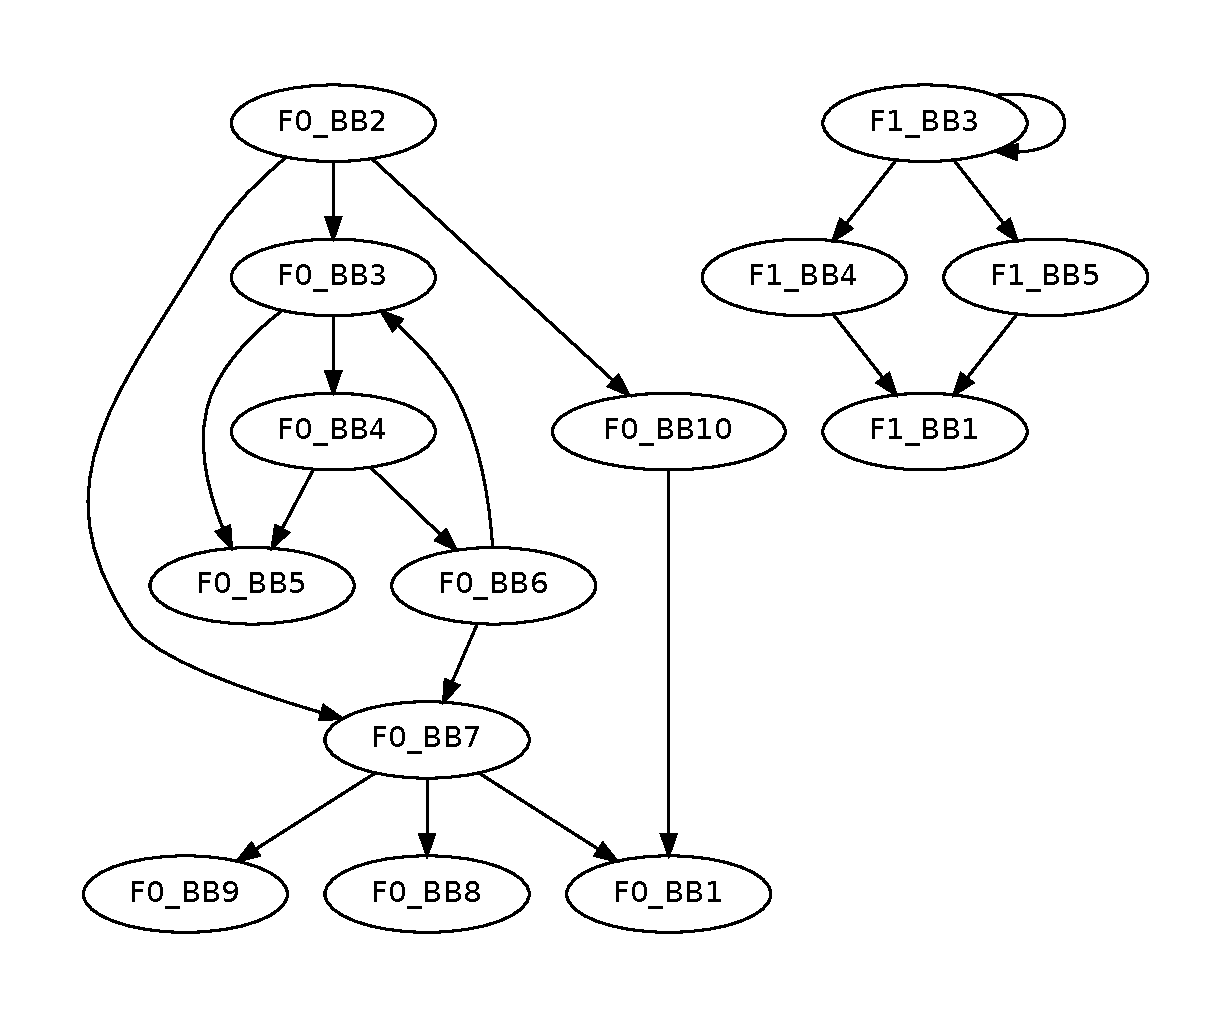
\includegraphics[scale=0.50]{images/t-test.pdf}
  \caption{Exemple de CFG d'une fonction}
  \label{fig:cfg}
\end{figure}


\newpage

\section{Construction du profiling}

L'objectif de cette partie était d'analyser et d'interpréter les traces de sortie d'exécution du code à compiler.\\

Nous avons donc développé un parseur LEX et YACC capable d'analyser les traces statiques et dynamiques issues du code instrumenté.\\

\subsection{Parsing LEX et YACC}

Les traces issues de l'instrumentation dynamique se présentent sous la forme suivante:
\begin{verbatim}
Appel X à la fonction main entrée cycle WW sortie cycle YY
Appel X à la fonction f1 entrée cycle WW sortie cycle YY
Appel X à la fonction f2 entrée cycle WW sortie cycle YY
\end{verbatim}

La grammaire reconnaissant les traces dynamiques est la suivante:
\begin{verbatim}
CALL FUNCTION NAME ENTERCYCLE NUMERIC EXITCYCLE NUMERIC RETLINE
\end{verbatim}

ENTERCYCLE et EXITCYCLE correspondent aux temps de début et de fin d'exécution d'une fonction.\\

\subsection{Profilage exclusif}

Le profilage issu du fichier de trace est inclusif, dans le sens où le temps total d'exécution d'une fonction inclut les temps d'exécution des fonctions appelées depuis la fonction parente.\\
L'analyse du fichier de traces se propose de produire un profilage exclusif, c'est-à-dire le temps d'exécution d'une fonction seule.\\

Pour pouvoir construire le profilage exclusif des fonctions, nous avions besoin de connaître les imbrications entre elles, et nous avons opté pour une construction sous forme d'arbres n-aires, où chaque noeud représente une fonction.\\

La première fonction analysée constitue la racine de l'arbre (il s'agira du point d'entrée \verb#main()# par exemple). Ensuite, pour chaque nouvelle fonction reconnue par l'analyseur, celui-ci créé un noeud qui est comparé aux noeuds précédents, en fonction des temps d'entrée et de sortie de la fonction.\\
Le noeud précédent le plus récent contenant une mesure d'entrée inférieure et une mesure de sortie supérieure au noeud dernièrement créé devient le parent de celui-ci. Le temps exclusif de la fonction parente est alors calculée en soustrayant son temps inclusif par le temps inclusif de la fonction enfant.\\

\begin{center}
  \begin{dot2tex}[neato,mathmode]
    digraph {
       label="main->exclusive time = main->inclusive time - func1->inclusive time"
      "main" -> "func1" 
      "func1" [style="fill=red!80"]
    }
  \end{dot2tex}
  \captionof{figure}{Add a first node}
\end{center}

Si un autre noeud ayant le même parent est ajouté, alors on soustrait à nouveau le temps exclusif du parent par le temps inclusif du nouveau noeud ajouté.\\

\begin{center}
  \begin{dot2tex}[neato,mathmode]
    digraph {
   label="main->exclusive time = main->exclusive time - func2->inclusive time"
   "main" -> "func1" 
   "main" -> "func2"
   "func2" [style="fill=red!80"]
    }
  \end{dot2tex}
  \captionof{figure}{Add a second node}
\end{center}

L'opération est répétée jusqu'à la fin de l'analyse du fichier de traces, jusqu'à obtenir le temps exclusif de toutes les fonctions.\\

\subsection{Gestion des instances}

L'un des objectifs du profiling est de pouvoir comparer les temps d'exécution de différentes instances d'une fonction.\\ 
Jusqu'à maintenant, tous les appels d'une même fonction sont chacun représentés par un noeud unique (on rajoute un noeud à chaque ligne lue par YACC).\\

\begin{center}
	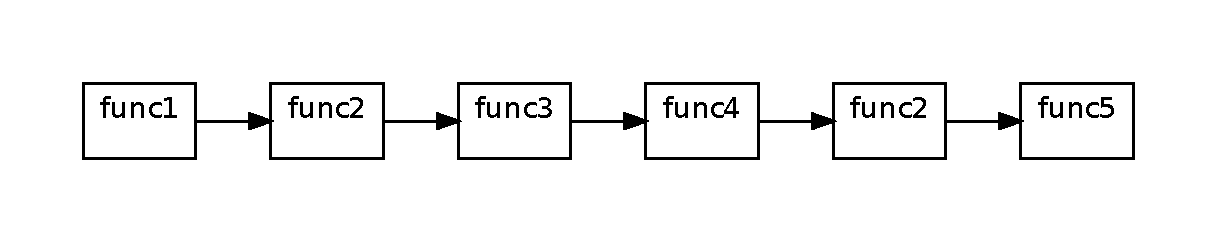
\includegraphics[scale=0.50]{images/liste1}
	\captionof{figure}{Nodes list}
\end{center}

Nous avons avant tout besoin de détecter les fonctions redondantes du fichier d'entrée, puis les considérer comme des instances différentes d'une même fonction.
Pour établir le nombre d'instances par fonction, l'analyseur reparcourt la liste des noeuds, identifie celles ayant le même nom, puis les stocke dans une structure, en renseignant le nombre d'instances.\\

\begin{center}
	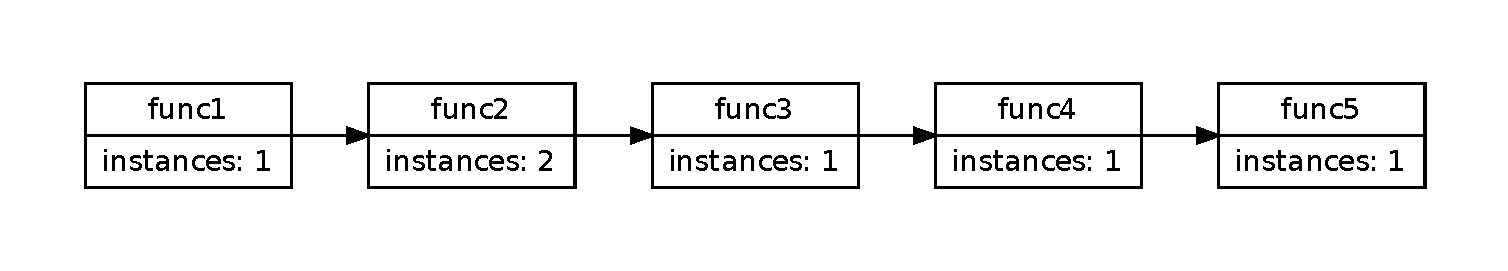
\includegraphics[scale=0.50]{images/ListIntances}
	\captionof{figure}{Nodes list with instances}
\end{center}

Les données recueillies sont ainsi sérialisées dans un fichier de sortie, puis interprétées en vue de produire un diagramme gnuplot \\

\subsection{Corrélation des instrumentations statique et dynamique}

La seconde partie du profiler consiste à corréler les données statiques et dynamiques d'une fonction, à savoir confronter le temps d'exécution et le nombre de load/store. Dans cette optique, nous avons construit une grammaire lui permettant de reconnaître les données issues de l'instrumentation statique:

\begin{verbatim}
FUNCTION NAME RETLINE
NUMERIC LOAD RETLINE
NUMERIC MUL NUMERIC LOAD RETLINE
NUMERIC STORE RETLINE
NUMERIC MUL NUMERIC STORE RETLINE
\end{verbatim}

Une fois les données statiques lues, on peut calculer le nombre de load et de store par fonction, puis, en parcourant la liste des fonctions déjà stockées, faire correspondre le nombre de load/store aux données dynamiques de la fonction précédemment analysée.\\

Une piste envisagée (qui a été implémentée), était de calculer une estimation de la latence d'un load et d'un store. Cette opération revenait à résoudre un système d'équations à deux inconnues (load et store), dont le résultat serait le temps d'exécution de la fonction concernée.\\
On résout le système en prenant en entrée un couple de fonctions, ce qui se traduit par:
\begin{verbatim}
load1*FacteurLoad1 + store1*FacteurStore1 = TempsFonction1
load2*FacteurLoad2 + store2*FacteurStore2 = TempsFonction2
\end{verbatim}
Système qui a été résolu en utilisant la méthode de Cramer.\\

L'opération a été répétée sur toutes les fonctions (en conservant la même fonction comme première équation), afin de calculer une moyenne sur les load/store.
Cependant, cette piste a été écartée en raison de la volatilité des latences d'accès mémoire.\\ 

\subsection{Graphe d'appel}

Enfin, le profiler propose la génération d'un graphe d'appel des fonctions, à l'aide d'un parcours préfixé de l'arbre n-aire construit. Il produit en sortie un fichier compréhensible par l'outil dot.

\begin{center}
	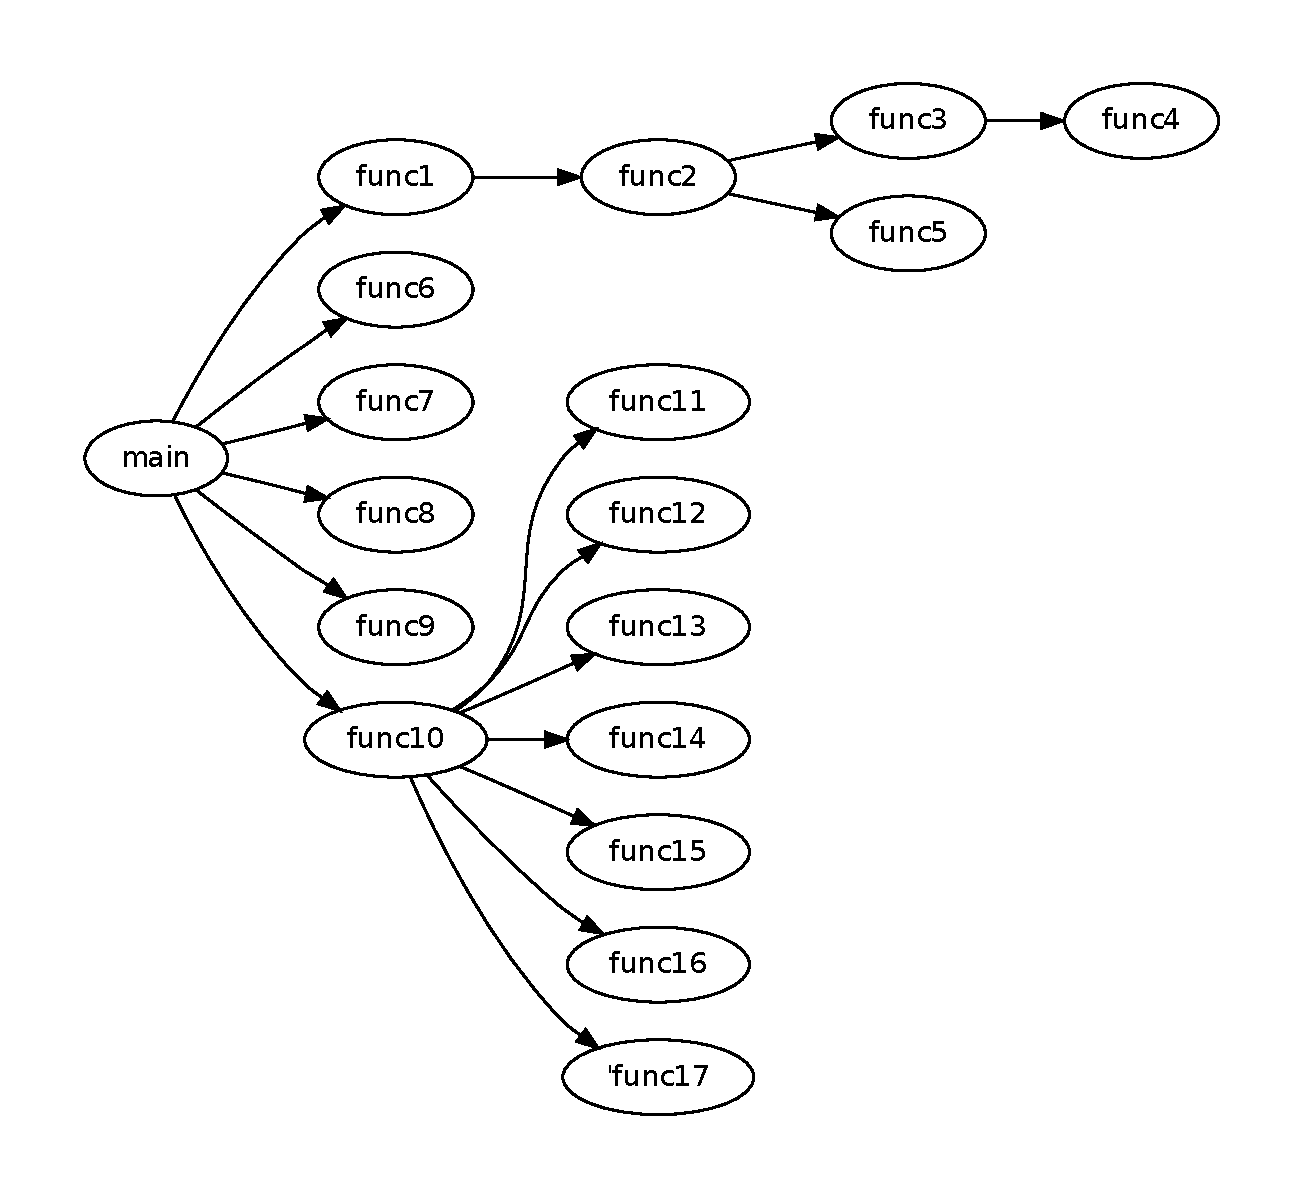
\includegraphics[scale=0.50]{images/CallGraph}
	\captionof{figure}{Functions Call Graph}
\end{center}




\newpage

% Permission is granted to copy, distribute and/or modify this document
% under the terms of the GNU Free Documentation License, Version 1.3
% or any later version published by the Free Software Foundation;
% with no Invariant Sections, no Front-Cover Texts, and no Back-Cover Texts.
% A copy of the license is included in the section entitled "GNU
% Free Documentation License".
%
% Authors:
% Caner Candan <caner@candan.fr>, http://caner.candan.fr
% Aurèle Mahéo <aurele.maheo@gmail.com>

\section{Multi-threading}

Un des problèmes qui peuvent se poser dans le cas d'une exécution multithreadée, est l'écriture concurrente sur les prises de mesure, faussant ainsi ces dernières.\\

Il est possible de remédier à ce problème en utilisant plusieurs techniques que nous citons:\\

\begin{itemize}

\item utilisation des mutexes\footnote{man pthreads} donnant droit à un accès exclusif aux données en écriture,\\

\item utilisation des POSIX semaphores\footnote{man sem\_overview} permettant une synchronisation des actions entre processus et threads,\\

\item utilisation du mot clé \verb#_thread# devant une déclaration de variable.\\

\end{itemize}


\newpage

\section{Réflexion sur le module de compilation}

Comme demandé, voici un avis critique (constructif nous l'espérons!) du module de compilation et de la manière dont les cours se déroulés.
Je dirais que les cours nous ont paru intéressants, ils nous ont permis de découvrir à quel point la compilation était une discipline dense, et qu'il n'était pas aisé de le couvrir en un laps de temps si court. Donc peu de choses à dire sur le contenu des cours.\\
Concernant les travaux dirigés, pas grand chose à dire non plus si ce n'est qu'il n'a pas été possible de tous les faire entièrement, problème de temps encore donc je ne vois pas grand chose à reprocher aux intervenants.\\
En revanche, je pense qu'il aurait été beaucoup plus simple de prendre connaissance du sujet du projet plus en avance, ce qui nous aurait permis une meilleure organisation, et nous aurait évité de devoir le mener "dans l'urgence", au détriment du reste. 	


\end{document}
